% template created by: Russell Haering. arr. Joseph Crop
\documentclass[12pt,letterpaper]{article}
\usepackage{anysize}
\usepackage{cite}
\usepackage{amsmath,amssymb,amsfonts}
\usepackage{algorithm}
\usepackage[noend]{algpseudocode}
\usepackage{graphicx}
\usepackage{multirow}
\usepackage{listings}
\usepackage{xcolor}


\marginsize{2cm}{2cm}{1cm}{1cm}

\lstset{ framexleftmargin=9mm, frame=shadowbox,tabsize = 4}

\begin{document}

\begin{titlepage}
    \vspace*{4cm}
    \begin{flushright}
    {\huge
        ECE 375 Lab 5\\[1cm]
    }
    {\large
    	External Interrupts
    }
    \end{flushright}
    \begin{flushleft}
    Lab session: 015
    
    Time: 12:00-13:50
    \end{flushleft}
    \begin{flushright}
    Author: Astrid Delestine

    Programming partner: Lucas Plastid 

    \vfill
    \rule{5in}{.5mm}\\
    TA Signature
    \end{flushright}

\end{titlepage}

\section{Introduction}
%This is the first Lab in the ECE 375 series and it covers the setup and compilation of an AVR Assembly Program. The student will learn how how to use the sample Basic Bump Bot assembly file and send the binaries to the AVR Microcontroller board. For the second part of the lab the student will be expected to download and compile the included C sample program and from it learn how to configure the I/O ports of the ATmega32U4 Microcontroller. The student will then write their own C program and upload it to the Microcontroller to verify that it runs as expected. The provided programs have been attached in the source code section of this report.
This is the Fifth lab in the ECE 375 series and it covers using hardware interrupts to preform predescribed "bump bot" operations. Additionally it incorporated use of the LCD Display to show the user how many times the bump bot had been triggered on its left or right side.

\section{Design}
In this lab Lucas and I setup several different interrupt vectors that were able to trigger certain functions. These functions made the program function similarly to the Lab 1 and 2 bump bot script. Once these interrupts were created and working we moved to creating counters and displays for each of the buttons pressed. In the image seen below, one can see an example of what the LCD display would look like upon boot up. 

\begin{figure}[h]
	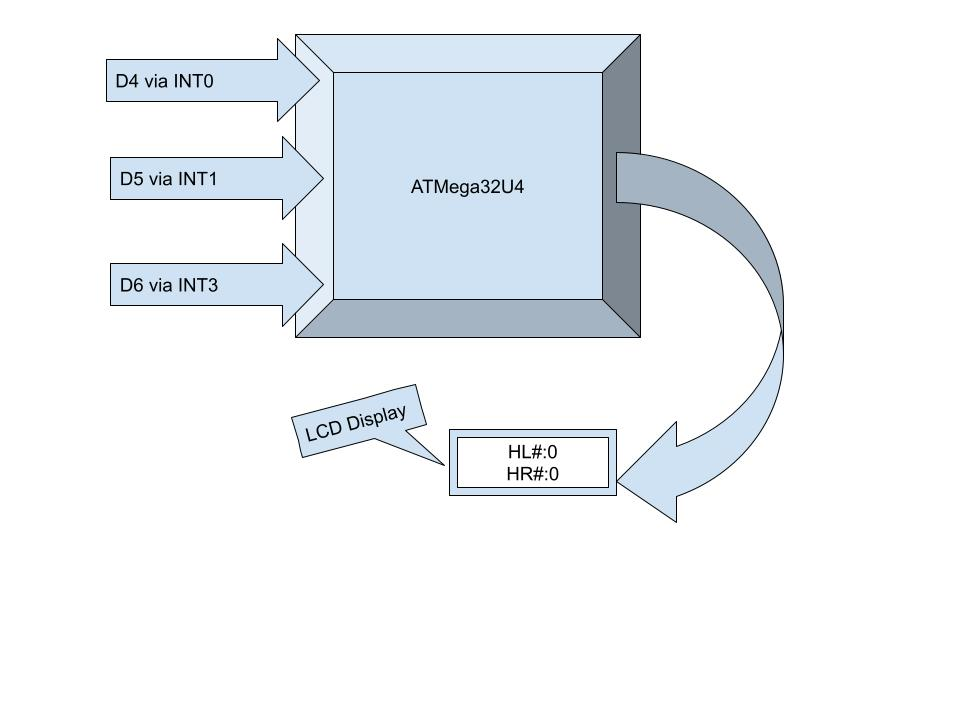
\includegraphics[width=12cm, height=10cm]{Block Diagram L5.jpg}
	\centering
\end{figure}
	
\section{Assembly Overview}
As for the Assembly program an overview can be seen below. 

\subsection{Internal Register Definitions and Constants}
Many different constants and registers are assigned in this program, and due to this they will not all be listed. Some more important registers will be highlighted however. The hlcnt and the hrcnt registers were created to count the number of times each button was pressed on either bumper. The strSize is a constant that determines how long the steady state numbers are that need to be patched in every time to the LCD are. All the other values and register assignments are either taken from Lab 1 or Lab 3 and connect to  the bump bot script or the LCD scripts.

\subsection{Interrupt Vectors}
Vectors setup are;
hit right on interrupt 0,
hit left on interrupt 1,
and clear counters on interrupt 3.



\subsection{Initialization Routine}
Firstly the stack pointer is initialized then ports B and D are initialized for output and input respectively. The LCD is then initialized in its own subroutines as we set it to turn its backlight on and clear any remaining text on the screen. Then we set it such that it displays clear delimiters for each of our button presses. Next we load up the interrupt control for falling edge detection, and configure the interrupt mask for just the 3 interrupts we had setup earlier. Finally we run the sei command to set the interrupt flag in SREG so that the interrupts can work at all.

\subsection{Main Routine}
The main routine is very simple due to the fact that most operations are handled outside of the main routine by interrupts. All it does is send the move forward command to the LEDs.


\subsection{Subroutines}
	\subsection{ClearCounters}
	This subroutine clears the counters for each button press, then clears the LCD of any overflowing numbers, and resets it back to its initial state. This is done by loading all 16 characters into the data memory that the display looks at for its characters.  
	
	\subsection{toLCD}
	The toLCD subroutine is quite simple with regards to what we have already completed. It sets the first four bits of each row to the characters in data memory then uses the built in Bin2ASCII command to take the mpr register and print it to the LCD display. It then enables the LCD to write the characters to the screen.

	\subsubsection{HitRight}
	This subroutine is nearly the same as the subroutine built for the original bump bot script. The major changes to it are that it increments a register such that it keeps track of how many times the subroutine is called, and it also calls the toLCD command, allowing the update to be pushed to the LCD. Finally it also has a debounce filter, to disable any interrupts that may have run during the method.
	 
	
	\subsubsection{HitLeft}
	This subroutine is nearly the same as the one built for the original bump bot script. It's major changes are the same as HitRight's, those being the associated counter, the toLCD command and the filter.
	
	\subsubsection{Wait}
	This is the stock wait function. It is unchanged from the original bump bot script.
	

\section{Testing}
Tested Each button press and compared to external calculations.
\begin{table}[h]
	\centering
	\begin{tabular}{|l|l|l|ll}
		\cline{1-3}
		Case & Expected & Actual meet expected &  &  \\ \cline{1-3}
	d4	&an increment on the LCD, and the bump bot right hit function to be called&	\checkmark  &  \\ \cline{1-3}
	d5	&an increment on the LCD, and the bump bot left hit function to be called&	\checkmark	&  \\ \cline{1-3}
	d6	&The two numbers listed on the screen reset&	\checkmark  &  \\ \cline{1-3}
	d7	&nothing&	\checkmark	&  \\ \cline{1-3}
	
%		&          &                      &  &  \\ \cline{1-3}
	\end{tabular}
\caption{Assembly Testing Cases}
\end{table}

\section{Study Questions}
\begin{enumerate}
    \item
    As this lab, Lab 1, and Lab 2 have demonstrated, there are always multiple ways to accomplish the same task when programming (this is especially true for assembly programming). As an engineer, you will need to be able to justify your design choices. You have now seen the BumpBot behavior implemented using two different programming languages (AVR assembly and C), and also using two different methods of receiving external input (polling and interrupts).
    Explain the benefits and costs of each of these approaches. Some important areas of interest include, but are not limited to: efficiency, speed, cost of context switching, programming time, understandability, etc.
    
    Each of these methods has its drawbacks and most of them have benefits. I will compare and contrast each of these starting from the least complex all the way to the most complex. Firstly C programming using busy waiting. This method is by far the easiest for the programmer to implement and understand what exactly is happening. The main downside for this method is its efficiency, speed, and size. It wins however when compared to all the others with regard to context switching, programming time, and understandability. 
    C programming with interrupts is the next step down the understandability ladder. Due to the average home programmer possibly being inexperienced, or unfamiliar with the ecosystem they are working on using interrupts in a C program will be a little bit more difficult than just using polling in their c program. The programming time, understandability, and ability to switch contexts will decrease when compared to a c program using polling, due to integration constrains and how each system implements their own interrupt systems differently. 
    As for assembly, only those who really know what they are doing can even begin to understand what is happening, so it would make sense to me that the polling version of this bump bot script is worse in every way but understandability. It takes less time to program, less space, and is more efficient, and faster to respond to changes. Understandability  falls by the wayside when working in assembly as it is the least important factor. as for portability, using any assembly code will need to change from one system to the next, so there is not that much more of a loss here in regards to that.
    
    
    \item 
    Instead of using the Wait function that was provided in BasicBumpBot.asm, is it possible to use a timer/counter interrupt to perform the one-second delays that are a part of the BumpBot behavior, while still using external
    interrupts for the bumpers? Give a reasonable argument either way, and be sure to mention if interrupt priority had any effect on your answer.
    
    It is possible as the priority of the timers is lower, they would have to be setup in such a way that they were allowed to run while the other interrupt is running. Or this is not possible due to the fact that they have a lower priority status. It truly depends on if the timer continues counting while the main function is interrupted. There is one other case, where the counter continues counting but will not reset without the interrupt, in this case, using an external interrupt timer would be feasible however a prescaler would need to be applied.
    
    \item 
    List the correct sequence of AVR assembly instructions needed to store the contents of registers R25:R24 into Timer/Counter1’s 16-bit register, TCNT1. (You may assume that registers R25:R24 have already been initialized to contain some 16-bit value.
    
 	
    (because its an IO location)

    in r25 TCNT1H
    in r24 TNCT1L
    
    \item
    List the correct sequence of AVR assembly instructions needed to load the contents of Timer/Counter1’s 16-bit register, TCNT1, into registers R25:R24
    
    out TCNT1H r25
	out TCNT1L r24
    
    \item 
    Suppose Timer/Counter0 (an 8-bit timer) has been configured to operate in Normal mode, and with no prescaling (i.e., clkT 0 = clkI/O = 8 MHz). The decimal value “128” has just been written into Timer/Counter0’s 8-bit
    register, TCNT0. How long will it take for the TOV0 flag to become set? Give your answer as an amount of time, not as a number of cycles
    
    it will take 16 microseconds
    
    
\end{enumerate}

\section{Difficulties}
This Lab challenged the thinking power of implementation of ideas we have learned in lecture. It was not too difficult however did require refrenceing both the AVR manual and the atmega32u4 datasheet.

\section{Conclusion}
In conclusion, this lab introduced and allowed the student to understand many more aspects of how to program a function using interrupts and modify an existing program to work with an LCD in conjunction with those interrupts. This lab proves that the student is learning how to modify certain code structures and is becoming more fluent in the AVR programming scheme

\pagebreak

\section{Source Code}%
\lstinputlisting
[
caption=Assembely Bump Bot Script,
language={[x86masm]Assembler},
numbers =left,
rulesepcolor=\color{blue}
]{../Lab5Assm/Lab5Assm/Lab5Assm/Astrid_Delestine_and_Lucas_Plaisted_Lab5_sourcecode.asm}





\end{document}